\textbf{COLUNI 2019 -- Questão 29}\par\medskip O heredograma a seguir representa uma família na qual estão indicados os alelos (“a” e “A”) para um gene relacionado a uma determinada doença, sendo que somente a mãe (Aa) não é doente.

% COLUNI-AUTO-FIGURES-BEGIN
\begin{figure}[htbp]
\centering
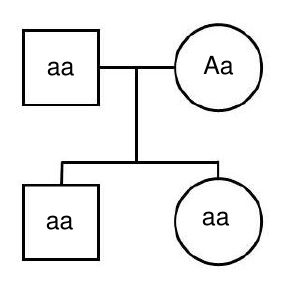
\includegraphics[width=0.95\linewidth]{static/simulados/coluni/figuras/2019/questao-29/figura-1.png}
\end{figure}
% COLUNI-AUTO-FIGURES-END

Sobre esse heredograma, assinale a afirmativa CORRETA:


\begin{enumerate}
\item A possibilidade de esse casal ter uma terceira criança doente é de 50\%.
\item Se a filha se casar com um homem doente, ela não terá filhos doentes.
\item Para ser doente, um indivíduo precisa ter herdado apenas um alelo recessivo.
\item O filho é doente por ter herdado o cromossomo X do pai.\end{enumerate}
